\documentclass{article}
\usepackage[utf8]{inputenc}
\usepackage[margin = 0.8in]{geometry}
\usepackage{graphicx}
\usepackage{amsmath, amssymb}
\usepackage{subcaption}
\usepackage{multirow}
\usepackage{mathtools}
\usepackage{float}


\title{RBE549 - Homework 2}
\author{Keith Chester}
\date{Due date: September 8, 2022}

\begin{document}
\maketitle

\section*{Problem 1}

In this problem, we attempt to prove with similar triangles that:

\begin{equation}
    \frac{1}{z_0} + \frac{1}{z_c} = \frac{1}{f}
\end{equation}

First, we look at the original diagram provided. I have added markers for the lengths ($z_0$ and $z_c$) assigned to their lengths, and marked the two lengths of $f$ to its distance from the center of the lens.

\begin{figure}[H]
    \centering
    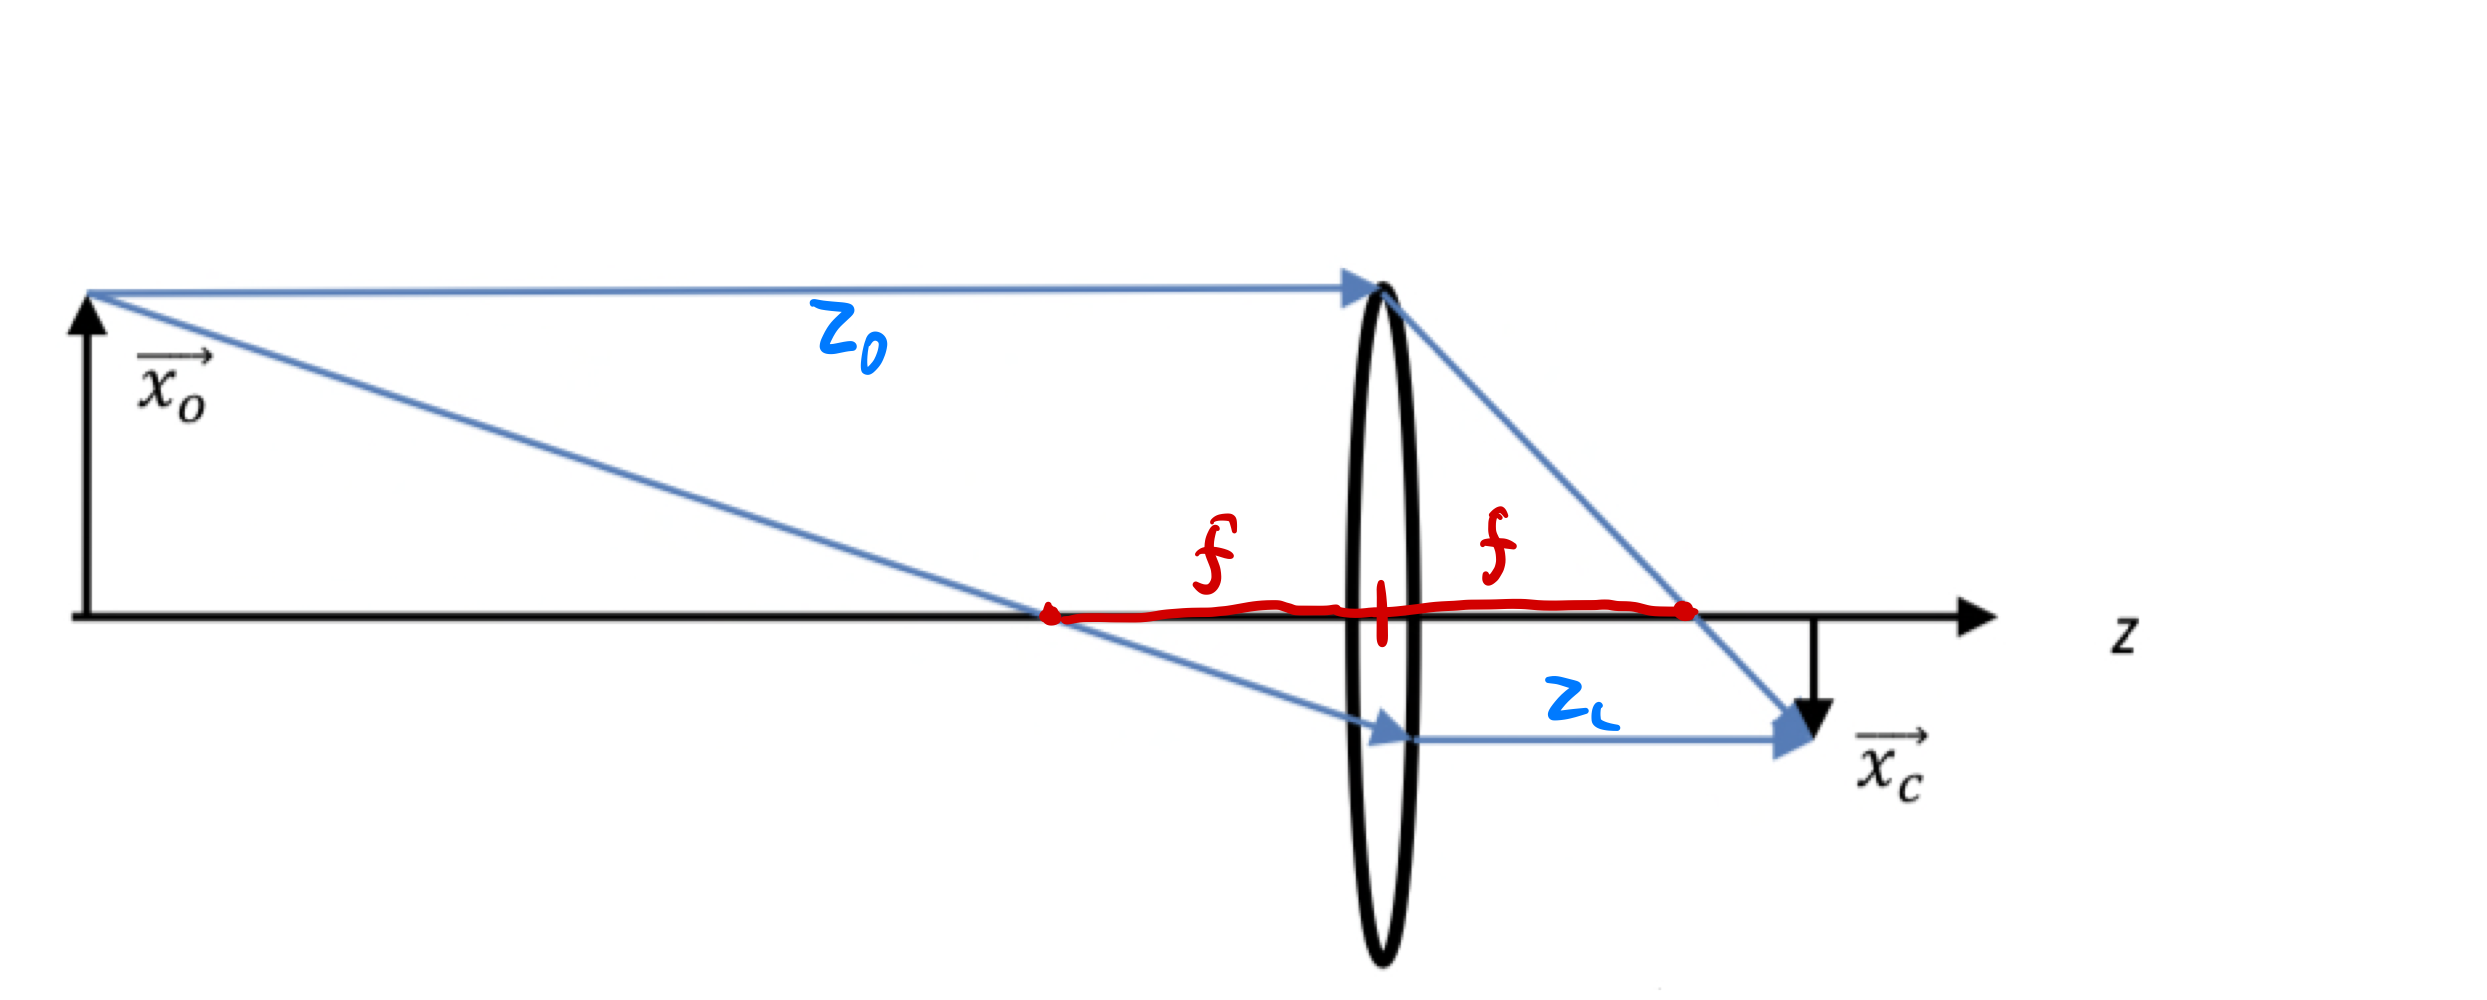
\includegraphics[width = 0.7\textwidth]{imgs/prob_1.png}
    \caption{Problem 1}
    \label{fig:prob1}
\end{figure}

We will note that the triangle provided by $z_0$ and be represented on the other side of the lens by flipping it along the lens as an axis. From there we can begin to mark angles.

\begin{figure}[H]
    \centering
    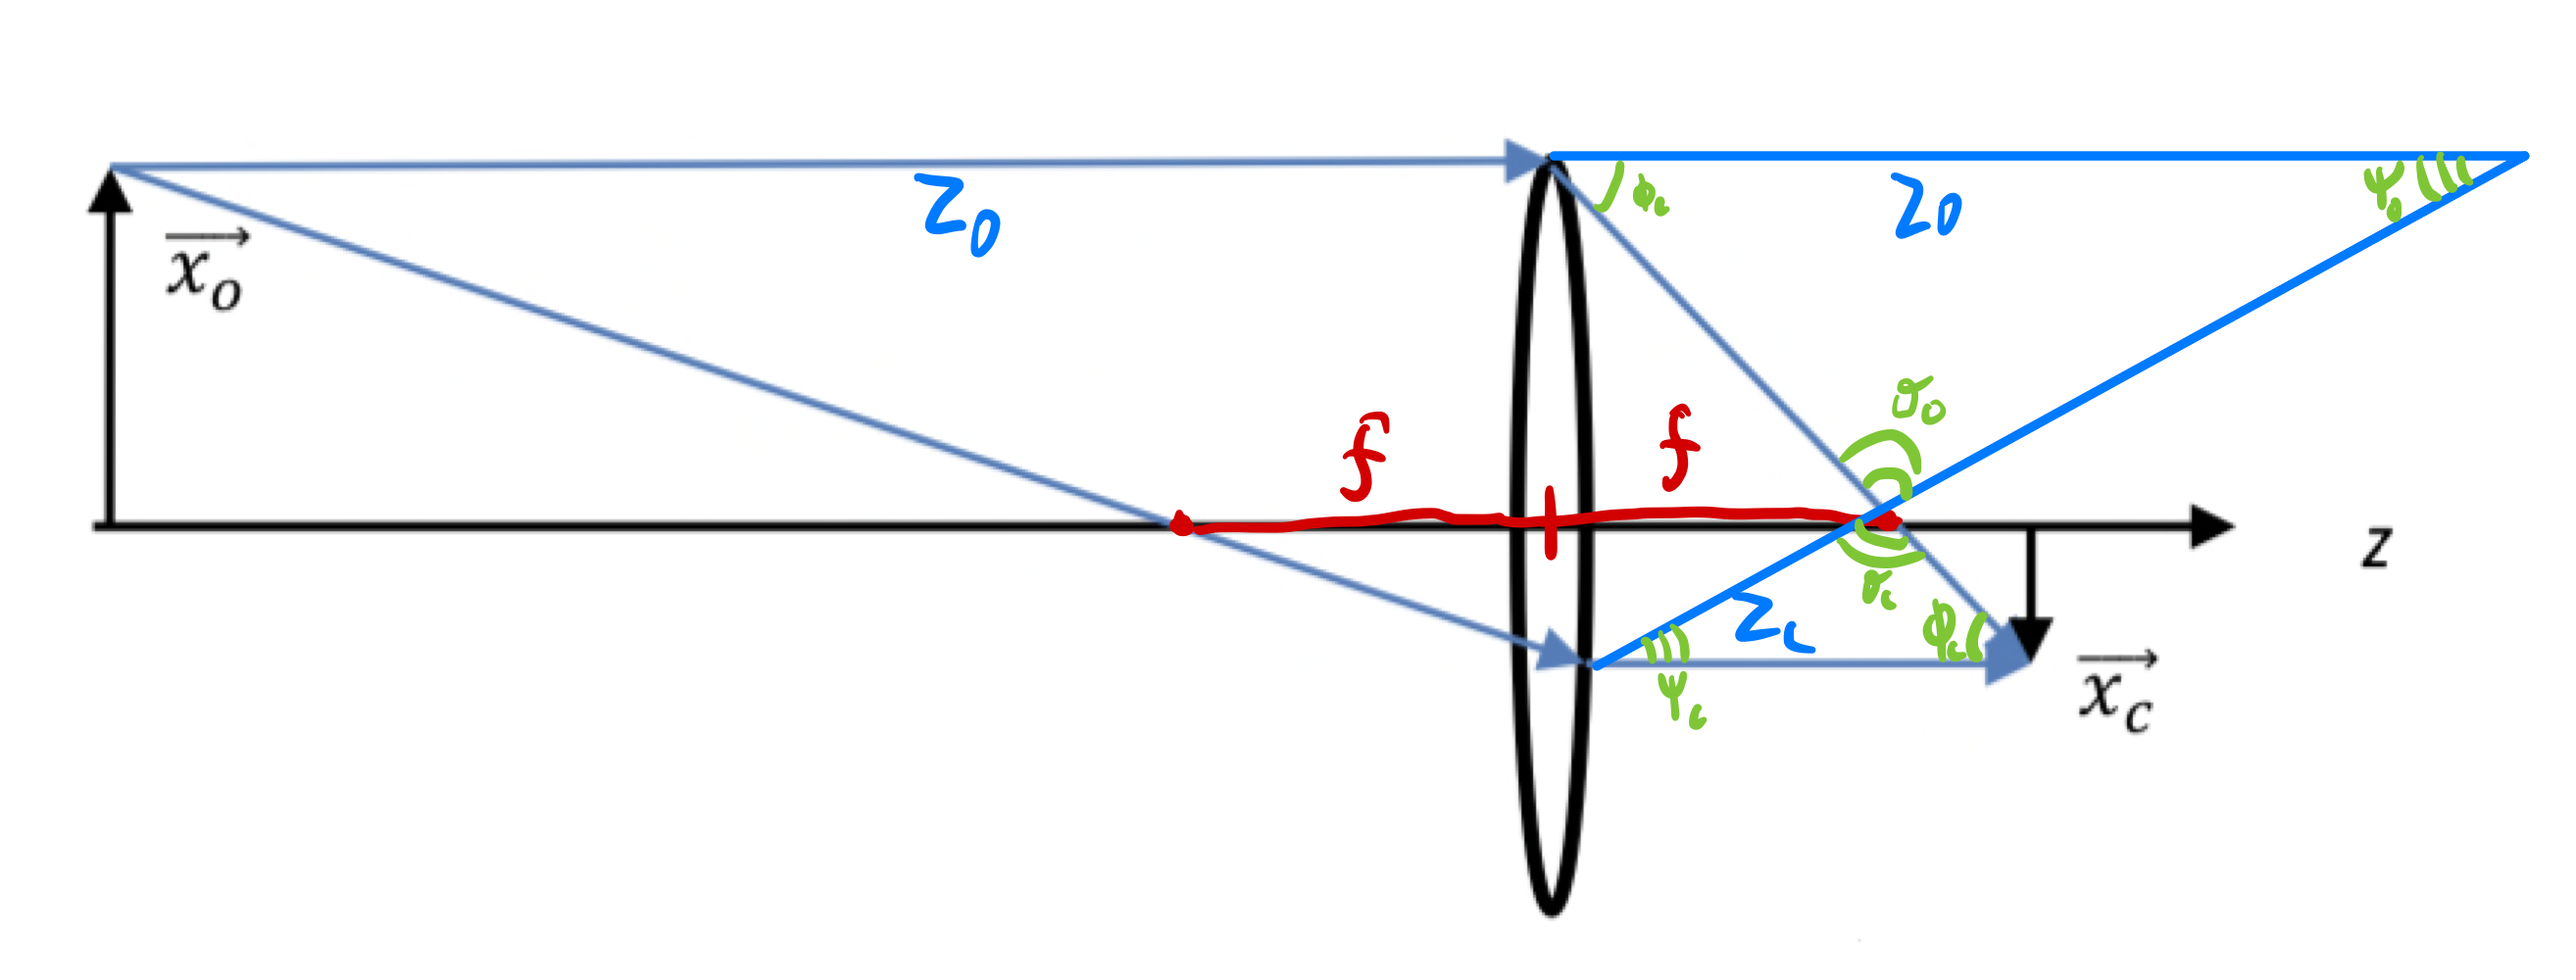
\includegraphics[width = 0.7\textwidth]{imgs/prob_1_expanded.png}
    \caption{Problem 1 Expanded}
    \label{fig:prob1_expanded}
\end{figure}

Because the $z$ access, $z_c$, and $z_0$ are parallel lines, we can thus know that opposite angles of lines crossing them are equivalent. Thus we see that $\phi_c$ and $\phi_0$ are equivalent and marked as such. Thesame goes for $\psi_c$ and $\psi_0$, as marked.  Since the lines passing through the focal point $f$ is rom parallel lines and continuous, we can also determine that $\theta_0$ and $\theta_c$ are also equivalent.

With this, we know that these are similar triangles, and can begin to form ratios to represent the relationships. Thus we have:

\begin{equation}
    \frac{z_0}{z_c} = \frac{f}{z_c - f}
\end{equation}

From here we can perform algebra to isolate the variables into a manner that is closer to what we sought to originally prove:

\begin{equation}
    z_0 z_c - z_0 f = z_c f
\end{equation}

\begin {equation}
    z_0 z_c = z_c f + z_0 f
\end{equation}

\begin{equation}
    z_0 z_c = f (z_c + z_0)
\end{equation}

\begin{equation}
    \frac{z_0 z_c}{f} = z_c + z_0
\end{equation}

\begin {equation}
    \frac{1}{f} = \frac{z_c + z_0}{z_0 z_c}
\end{equation}

\begin{equation}
    \frac{1}{f} = \frac{z_c}{z_0 z_c} + \frac{z_0}{z_0 z_c}
\end{equation}

\begin{eqnarray}
    \frac{1}{f} = \frac{1}{z_0} + \frac{1}{z_c}
\end{eqnarray}

\section*{Problem 2}

\subsection*{A}
A typical human eyeball is $2.4cm$ in diameter and contains roughly $150,000,000$ receptors. Assuming a uniform distribution of receptors across the hemisphere, how many receptors are there per $mm^2$?

\begin{equation}
    \text{Area of hemisphere} = \frac{1}{2}4\pi r^2 = 2\pi r ^2
\end{equation}

\begin{equation}
    = 2 \pi (\frac{0.24}{2}) ^2 = 2 \pi 0.12^2 = 904.78 mm
\end{equation}

\begin{equation}
    \frac{150,000,000}{904.78} \approx 165,786
\end{equation}

So with these assumptions there are approximatley $165,786$ receptors per $mm^2$.

\subsection*{B}

In this problem, we put forth that mars mars has a diameter of $8,000km$ and an average distance from Earth of $225,000,000km$. Using a value of f equal to the eye's diameter, on how many receptors does the image of Mars fall?

We can use similar triangles, as we did in problem one, to create a ratio which we can use to determine the size of the image of Mars on our eye, and from this determine the number of receptors that see Mars. The ratio we ultimately aim to achieve first is:

\begin{equation}
    \frac{z_0}{z_c} = \frac{h_0}{h_1}
\end{equation}


...but what is $z_c$?

As we saw earlier, we can use:

\begin{equation}
    \frac{1}{f} = \frac{1}{z_0} + \frac{1}{z_c}
\end{equation}

\begin{equation}
    \frac{1}{2.4cm} = \frac{1}{225,000,000km} + \frac{1}{z_c}
\end{equation}

\begin{equation}
    z_c = 2.4cm
\end{equation}

...Which is a barely noticeable value smaller than our given focal length. With this, we can now set up our ration of image sizing:

\begin{equation}
    \frac{8,000km}{h_i} = \frac{225,000,000km}{2.4cm}
\end{equation}

...and the height/diameter of our mars image is thus:

\begin{equation}
    h_i = 8.53*10^{-7}m
\end{equation}

Multiplied by our receptors per $mm$ caluclated earlier:

\begin{equation}
    8.53*10^{-7} \times 165,786 \approx 0.141 \text{ receptors}
\end{equation}

...this results in less than one receptor receiving the light of mars, which means we can't see it normally with our eyes alone.

\section*{Problem 3}

An image has object and backgronud pixels whose brightness values are distributed in accodance to a Gaussian (normal) distribution with the same mean $\mu$ but different variances $\sigma_0$ and $\sigma_b$ with $\sigma_o < \sigma_b$.

\begin{equation}
    P_o(x-\mu) > P_b(x-\mu)
\end{equation}

It is desired to segment the image into object and background. To this end we wish to show that the decision rule that maximizes the probability of a correct decision is to label each pixel with brightness x as \textit{object} or \textit{background}:

\begin {equation}
    \frac{1}{\sqrt{2\pi}\sigma_o}e^{\frac{-(x-\mu)^2}{2\sigma^2_o}} > \frac{1}{\sqrt{2\pi}\sigma_b}e^{\frac{-(x-\mu)^2}{2\sigma^2_b}}
\end{equation}

First we will try to isolate our terms by taking the natural log. Since $ln(ab) = ln(a) + ln(b)$ and $ln(\frac{a}{b}) = ln(a) - ln(b)$...:

\begin{equation}
    \ln(1) - \ln(\sqrt{2\pi}\sigma_o) + \frac{-(x-\mu)^2}{2\sigma^2_o} > \ln(1) - \ln(\sqrt{2\pi}\sigma_b) + \frac{-(x-\mu)^2}{2\sigma^2_b}
\end{equation}

\begin{equation}
    \ln(\sigma_b) - \ln(\sigma_o) > \frac{-(x-\mu)^2}{2\sigma^2_o} - \frac{-(x-\mu)^2}{2\sigma^2_b}
\end{equation}

\begin{equation}
    \ln(\sigma_b) - \ln(\sigma_o) > \frac{((x-\mu)^2 2\sigma_b^2 - ((x-\mu)^2 2\sigma_o^2 }{2\sigma^2_o2 \sigma^2_b2}
\end{equation}

\begin{equation}
    (\ln(\sigma_b) - \ln(\sigma_o)) (2\sigma^2_o2 \sigma^2_b2)  > ((x-\mu)^2 2\sigma_b^2) - ((x-\mu)^2 2\sigma_o^2)
\end{equation}

\begin{equation}
    \frac{(\ln(\sigma_b) - \ln(\sigma_o)) (2\sigma^2_o2 \sigma^2_b2)}{\sigma_b^2 - \sigma_o^2} > (x - \mu)^2
\end{equation}

...and finally we can finalize this result by taking the square root of above, resulting in:

\begin{equation}
    \sigma_b \sigma_o \sqrt{\frac{\ln(\sigma_b) - \ln(\sigma_o)}{\sigma_b^2 \sigma_o^2}} > \vert x - \mu \vert
\end{equation}

\section*{Problem 4}

In this problem, we look at the inverse of a transformation matrix, $H$, where:

\begin{equation}
    H = \begin{bmatrix}
        \boldsymbol{R} & \vdots & T \\
        \dots & & \dots \\
        0 & \vdots & 1 \\
    \end{bmatrix}
\end{equation}

The true inverse of a transformation matrix is:

\begin{equation}
    H^{-1} = \begin{bmatrix}
        \boldsymbol{R}^T & \vdots & -\boldsymbol{R}^T T \\
        \dots & & \dots \\
        0 & \vdots & 1 \\
    \end{bmatrix}
\end{equation}

This additional step is needed as the translation from the original point is influenced by the orientation of the previous transform; therefore we must perform a translation that also considers reversing the affected rotation as well.

\section*{Problem 5}

In this problem, we attempt to create a binary threshold of a selfie image in order to demonstrate thresholding. The image in question is below.

\begin{figure}[H]
    \centering
    \includegraphics[width = 0.7\textwidth]{selfie.jpg}
    \caption{Pop up dinner selfie}
    \label{fig:selfie}
\end{figure}

\subsection*{A}

In this section, we use OpenCV to open the image and convert it to grayscale. Once we have the image in grayscale, we ask OpenCV to create a histogram of bins, where each possible pixel value (from $0$ to $255$, or one byte) is a bin. From here, we check how many of the pixels exist in each bin. Once we have hit $80\%$ of the image's pixels being set to white, we are done.

The code for this can be viewed in \textit{problem\_5a.py}. Below is the image generated from the code.

\begin{figure}[H]
    \centering
    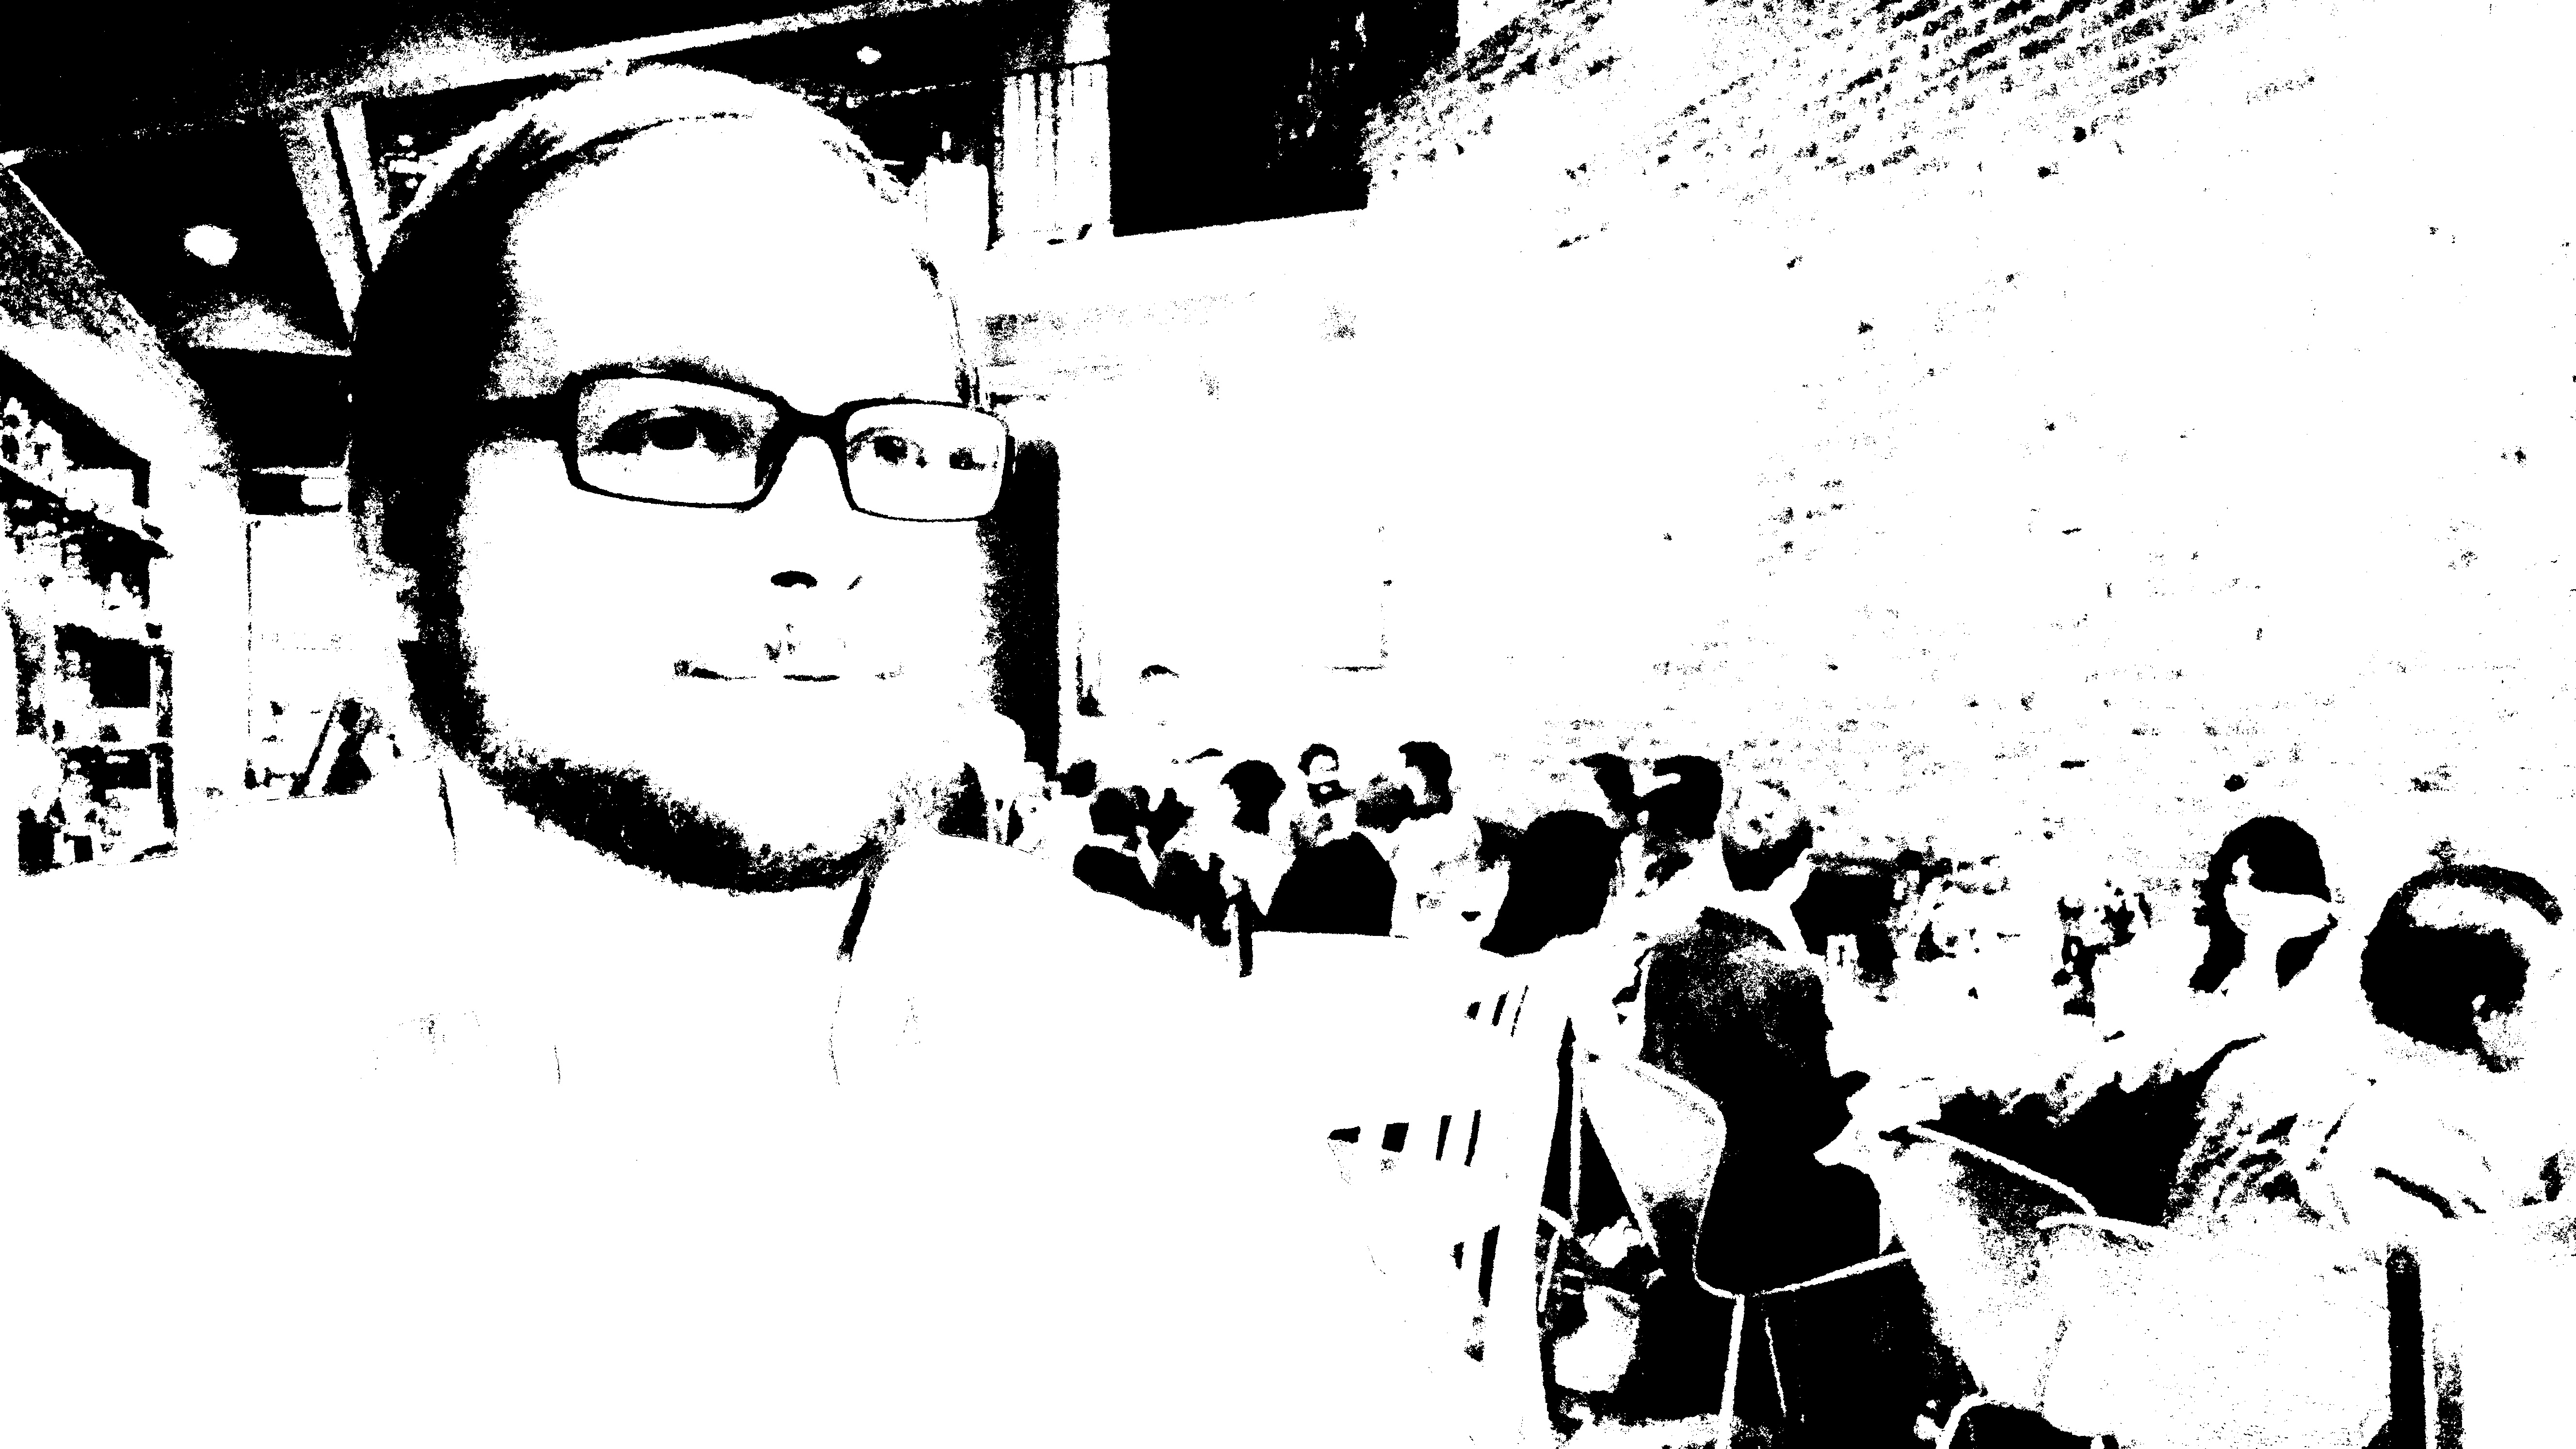
\includegraphics[width = 0.7\textwidth]{imgs/binary_threshold.jpg}
    \caption{Binary Threshold}
    \label{fig:problem5a}
\end{figure}

\subsection*{B}

For this section, we wish to experiment with other thresholding types. The code for this can be viewed in \textit{problem\_5b.py}. Instead of building the threshold out manaully, we use OpenCV's built in thresholding functions. We demonstrate a straight binary threshold (similar to what we did before, but with a cutoff value of $127$, or half max intensity) and then a mean and gaussian adaptive threshold. These methods are utilized to demonstrate common methods that one would have already prepared for them in the toolbox of OpenCV. Note that I performed a gaussian blur on the image prior as well, in hopes to reduce noise on these thresholding functions.

\begin{figure}[H]
    \centering
    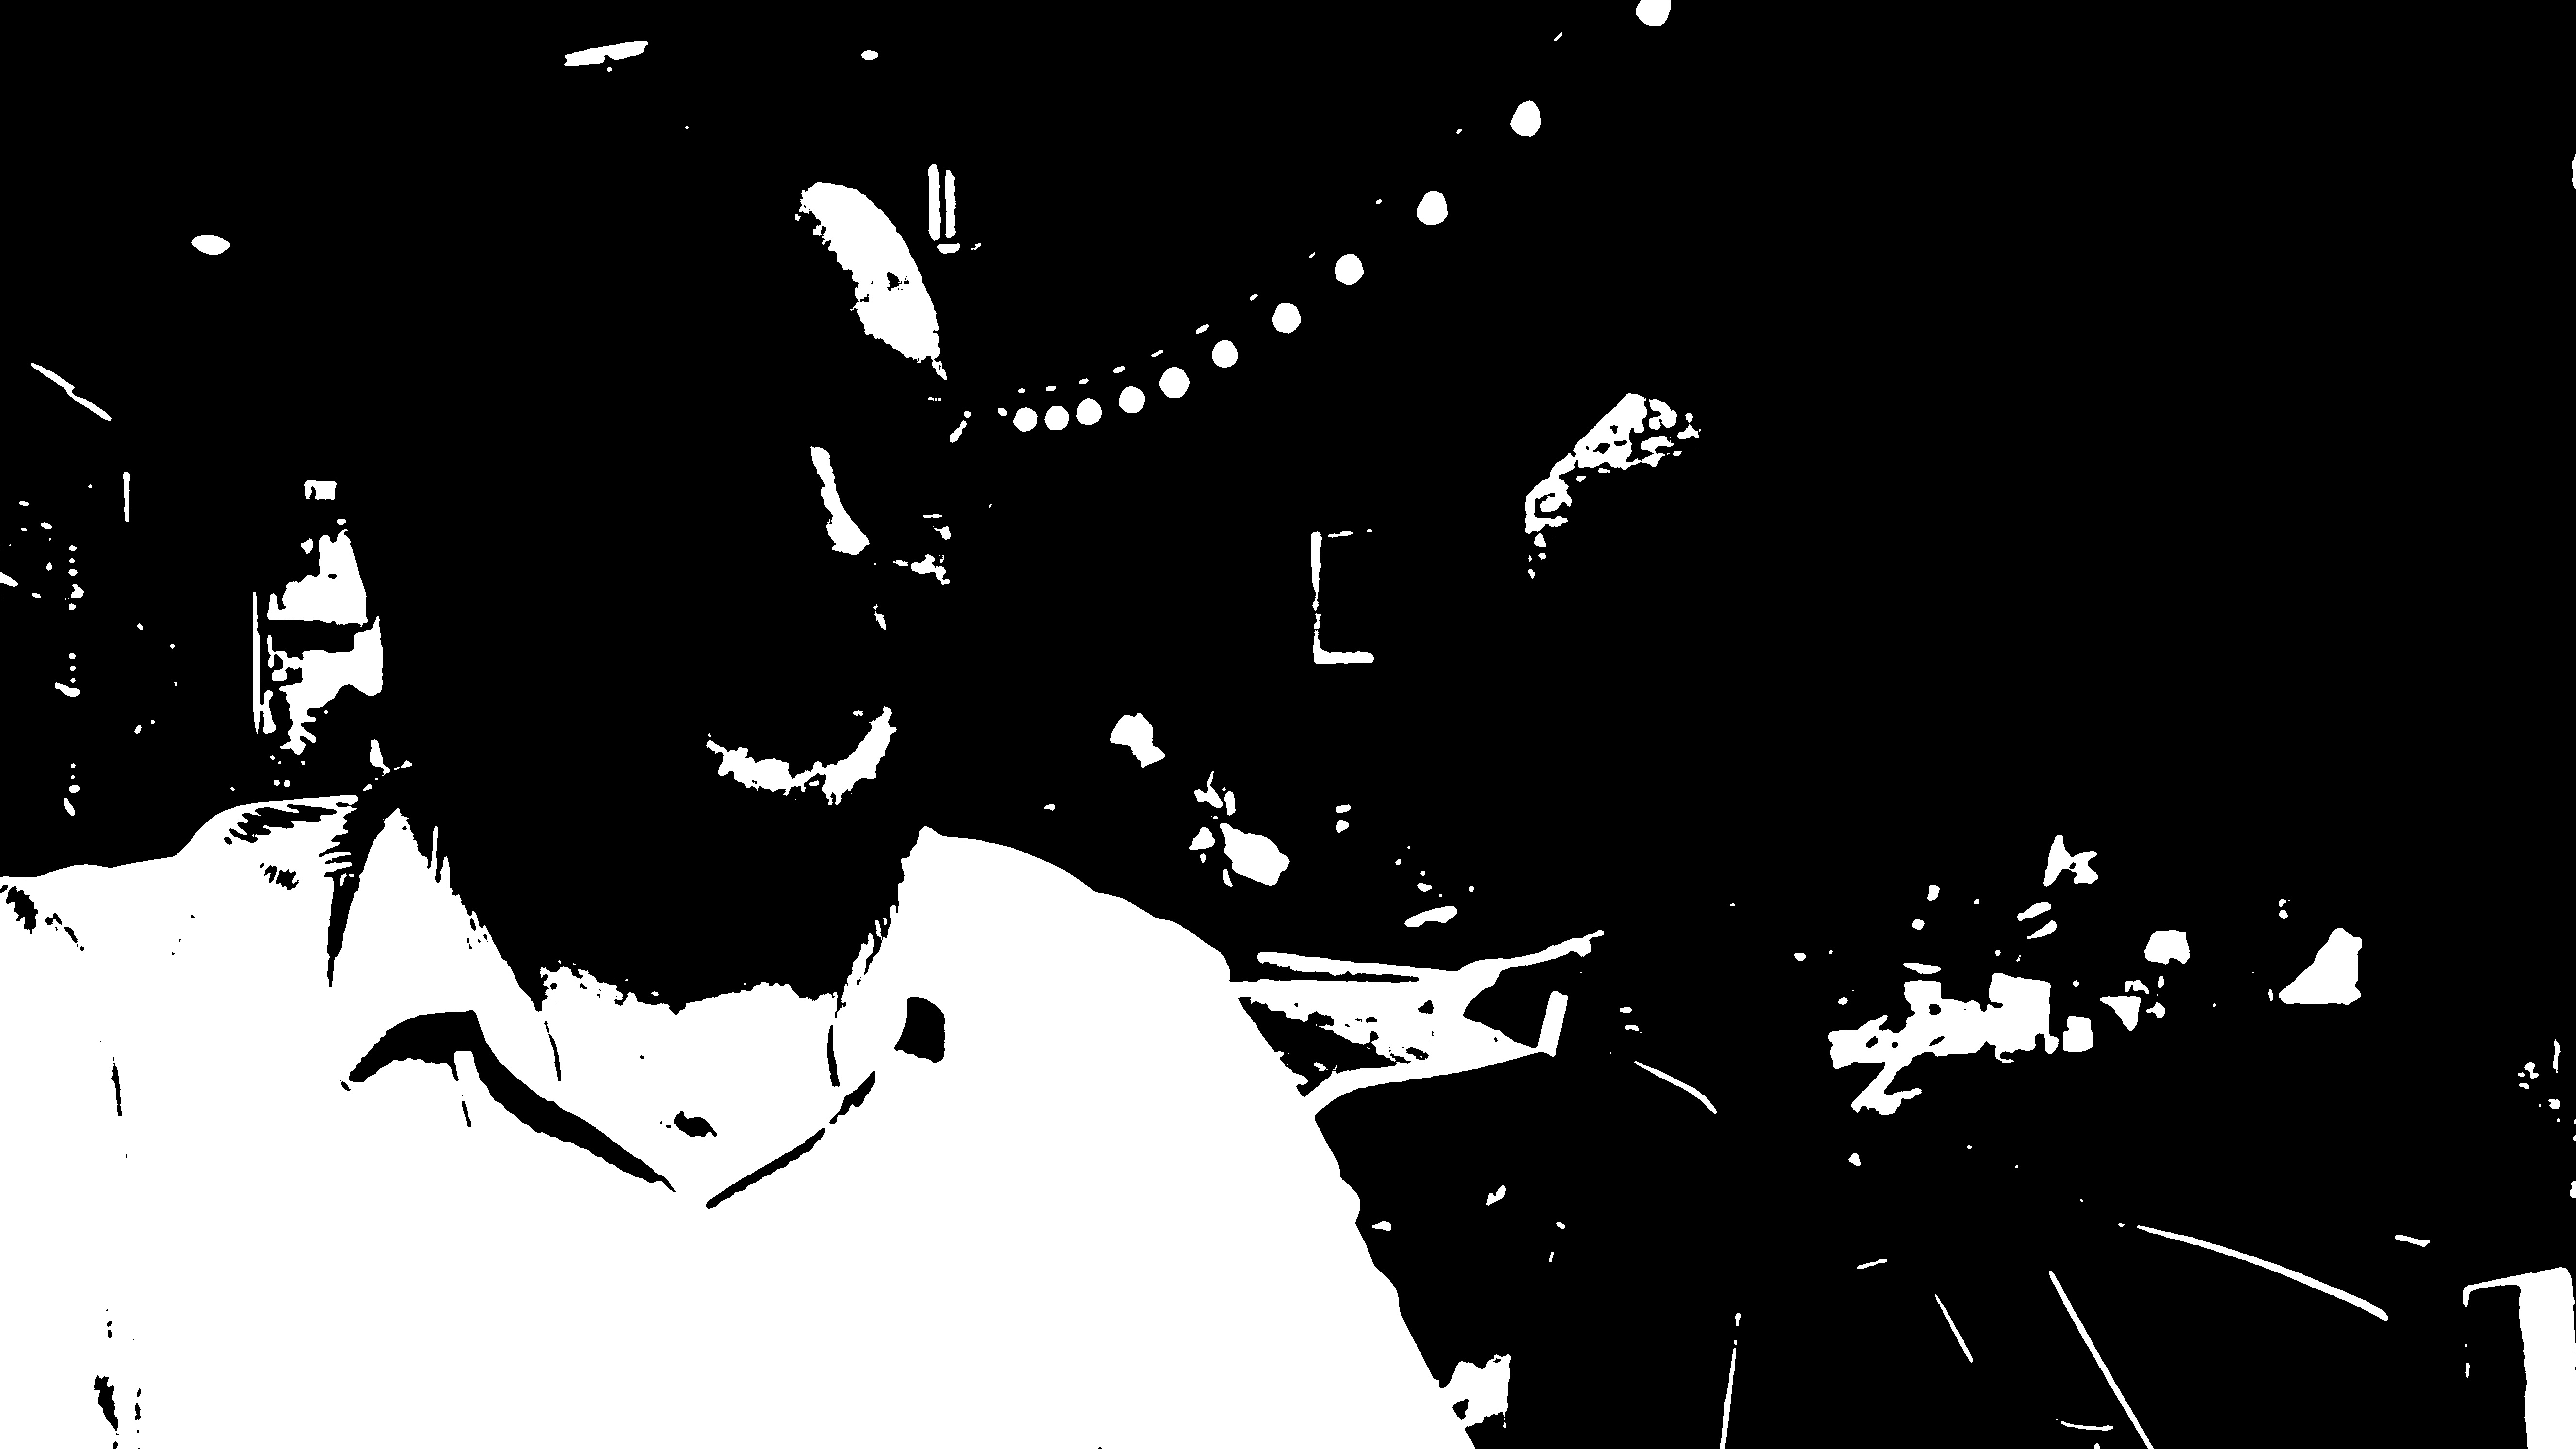
\includegraphics[width = 0.7\textwidth]{imgs/5b_binary_threshold.jpg}
    \caption{Binary Threshold}
    \label{fig:problem5b1}
\end{figure}

\begin{figure}[H]
    \centering
    \includegraphics[width = 0.7\textwidth]{imgs/5b_adaptive_threshold_mean.jpg}
    \caption{Adaptive Threshold - Mean Blur}
    \label{fig:problem5b2}
\end{figure}

\begin{figure}[H]
    \centering
    \includegraphics[width = 0.7\textwidth]{imgs/5b_adaptive_threshold_gaussian.jpg}
    \caption{Binary Threshold - Gaussian Blur}
    \label{fig:problem5b3}
\end{figure}

\end{document}